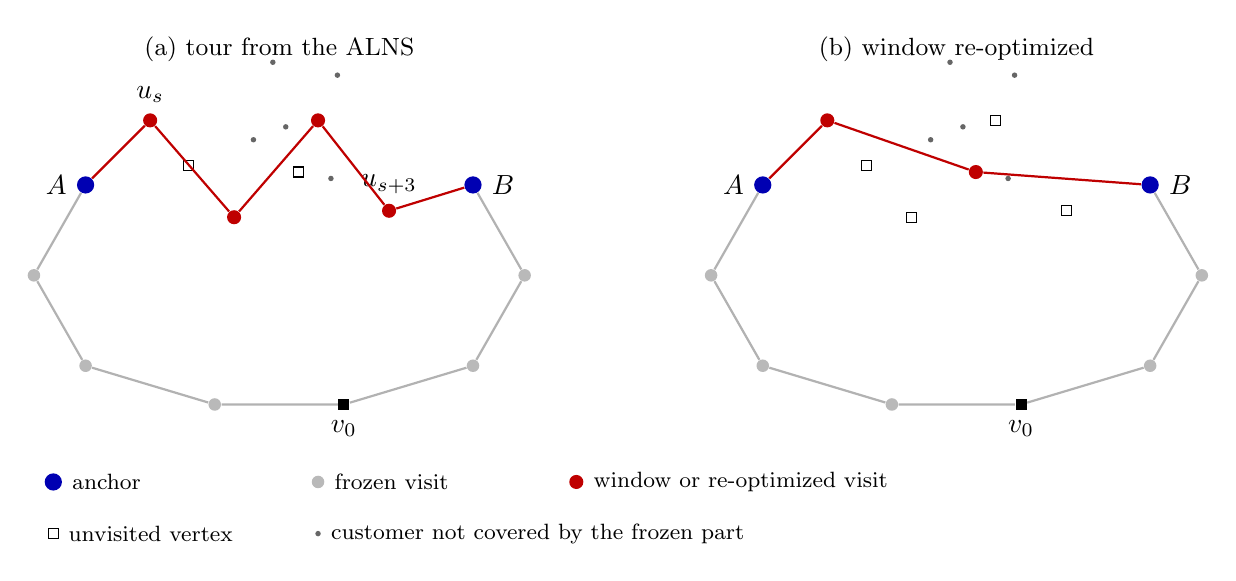
\begin{tikzpicture}[x=0.82cm,y=0.82cm,
  frozen/.style={circle,fill=gray!55,inner sep=1.6pt},
  anc/.style={circle,fill=blue!70!black,inner sep=2.2pt},
  win/.style={circle,fill=red!75!black,inner sep=1.8pt},
  cand/.style={rectangle,draw=black,fill=white,inner sep=1.8pt},
  depot/.style={rectangle,fill=black,inner sep=2pt},
  cust/.style={circle,fill=black!60,inner sep=0.7pt}]
% ---------- panel (a): tour before polishing
\begin{scope}
\node[font=\small] at (1,4.1) {(a) tour from the ALNS};
\node[anc,label=left:{$A$}] (A) at (-2,2) {};
\node[anc,label=right:{$B$}] (B) at (4,2) {};
\node[frozen] (f1) at (4.8,0.6) {};
\node[frozen] (f2) at (4.0,-0.8) {};
\node[depot,label=below:{$v_0$}] (f3) at (2,-1.4) {};
\node[frozen] (f4) at (0,-1.4) {};
\node[frozen] (f5) at (-2,-0.8) {};
\node[frozen] (f6) at (-2.8,0.6) {};
\node[win,label=above:{$u_s$}] (w1) at (-1,3.0) {};
\node[win] (w2) at (0.3,1.5) {};
\node[win] (w3) at (1.6,3.0) {};
\node[win,label=above:{$u_{s+3}$}] (w4) at (2.7,1.6) {};
\node[cand] (c1) at (1.3,2.2) {};
\node[cand] (c2) at (-0.4,2.3) {};
\draw[gray!60,thick] (B)--(f1)--(f2)--(f3)--(f4)--(f5)--(f6)--(A);
\draw[red!75!black,thick] (A)--(w1)--(w2)--(w3)--(w4)--(B);
\foreach \p in {(0.9,3.9),(1.9,3.7),(1.1,2.9),(0.6,2.7),(1.8,2.1)} \node[cust] at \p {};
\end{scope}
% ---------- panel (b): tour after polishing
\begin{scope}[xshift=8.6cm]
\node[font=\small] at (1,4.1) {(b) window re-optimized};
\node[anc,label=left:{$A$}] (A) at (-2,2) {};
\node[anc,label=right:{$B$}] (B) at (4,2) {};
\node[frozen] (f1) at (4.8,0.6) {};
\node[frozen] (f2) at (4.0,-0.8) {};
\node[depot,label=below:{$v_0$}] (f3) at (2,-1.4) {};
\node[frozen] (f4) at (0,-1.4) {};
\node[frozen] (f5) at (-2,-0.8) {};
\node[frozen] (f6) at (-2.8,0.6) {};
\node[win] (w1) at (-1,3.0) {};
\node[win] (c1) at (1.3,2.2) {};
\node[cand] (w2) at (0.3,1.5) {};
\node[cand] (w3) at (1.6,3.0) {};
\node[cand] (w4) at (2.7,1.6) {};
\node[cand] (c2) at (-0.4,2.3) {};
\draw[gray!60,thick] (B)--(f1)--(f2)--(f3)--(f4)--(f5)--(f6)--(A);
\draw[red!75!black,thick] (A)--(w1)--(c1)--(B);
\foreach \p in {(0.9,3.9),(1.9,3.7),(1.1,2.9),(0.6,2.7),(1.8,2.1)} \node[cust] at \p {};
\end{scope}
% ---------- legend
\node[anc,label=right:{\footnotesize anchor}] at (-2.5,-2.6) {};
\node[frozen,label=right:{\footnotesize frozen visit}] at (1.6,-2.6) {};
\node[win,label=right:{\footnotesize window or re-optimized visit}] at (5.6,-2.6) {};
\node[cand,label=right:{\footnotesize unvisited vertex}] at (-2.5,-3.4) {};
\node[cust,label=right:{\footnotesize customer not covered by the frozen part}] at (1.6,-3.4) {};
\end{tikzpicture}
